\documentclass[10pt,A4paper]{article}

\usepackage{acronym}
\usepackage{amsmath,amssymb}
\usepackage[aboveskip=1pt,labelfont=bf,labelsep=period,justification=raggedright,singlelinecheck=off]{caption}
\usepackage{changepage}
\usepackage{cite}
\usepackage{nameref,hyperref}
\usepackage[right]{lineno}
\usepackage[nopatch=eqnum]{microtype}

\usepackage{xcolor}
\usepackage{multirow}
\usepackage{ctable} % for \specialrule command
\usepackage{graphicx}
\usepackage{subcaption}

\usepackage[outputdir=out]{minted}
\definecolor{bg}{HTML}{282828} % fro https://github.com/kevinsawicki/monokai
\setminted{autogobble=true,bgcolor=bg,linenos=true,style=monokai}

\bibliographystyle{abbrv}

% Header and Footer with logo
\usepackage{lastpage,fancyhdr,graphicx}
\usepackage{epstopdf}
\pagestyle{fancy}
\fancyhf{}
\rfoot{\thepage/\pageref{LastPage}}
\renewcommand{\headrulewidth}{0pt}
\renewcommand{\footrule}{\hrule height 2pt \vspace{2mm}}
\lfoot{\today}

\newcommand{\etal}{{\textit{et al. }}}
\newcommand{\mbx}{\mathbf{x}}
\newcommand{\mbu}{\mathbf{u}}
\newcommand{\mbp}{\mathbf{p}}
\newcommand{\mby}{\mathbf{y}}
\providecommand{\keywords}[1]{\textbf{Keywords } #1}

% Create a new environment for code samples.
\newfloat{code}{tbp}{lop}
\floatname{code}{Code Sample}


% Create acronyms to use in text
\newacro{ode}[ODE]{Ordinary Differential Equation}
\newacro{oed}[OED]{optimal experimental design}
\newacro{fim}[FIM]{Fisher information matrix}
\newacro{de}[DE]{Differential evolution}


\begin{document}
% ########################################################################
% ########################################################################
\vspace*{0.2in}
% Title must be 250 characters or less.
\begin{flushleft}
{\Large
\textbf\newline{Model Calibration with Process Variables depending on Environmental Parameters}}
\newline
\\
Polina Gaindrik\textsuperscript{1,2,3},
Jonas Pleyer\textsuperscript{1,2},
Christian Fleck\textsuperscript{1,2,3}
\\
\bigskip
\textbf{1} \href{https://www.fdm.uni-freiburg.de/spatsysbio}{University of Freiburg}\\
\textbf{2} \href{https://www.fdm.uni-freiburg.de/spatsysbio}{Freiburg Center for Data Analysis and Modeling}\\
\textbf{3} \href{https://tsenso.com/en/}{tsenso GmbH}\\
\bigskip

\end{flushleft}
% ########################################################################
% ########################################################################
\section*{Abstract}
\linenumbers
Parameter estimation is a significant part of the model building that is always accompanied by uncertainty.
Experimental design allows optimization of the observation conditions and reduces the uncertainty of the parameter estimation as well as the number of measurements required for meaningful model quantification.
In this chapter, we provide instructions for finding the optimal experimental design using the Baranyi and Roberts growth model with the 'square root' secondary model for the maximum growth rate as a specific example from Predictive Microbiology. 
The guidelines are supposed to clarify the procedure and make it more accessible for the reader familiar with the field of Systems Biology.
We provide Python-written software FisInMa for the \acp{ode}-based models that optimize the measurement times and inputs of the model.


\keywords{Optimal experimental design, Parameter estimation, Fisher Information matrix, Identifiability, Uncertainty}

%
%
%
% ########################################################################
% ########################################################################
\section*{Introduction}
% \begin{figure}[h]
% 	\inputminted[linenos,firstline=57,lastline=79]{python}{../model-design-fischer-information-matrix/pool_model.py}
% 	\caption{Sample code written in Python~\cite{rossumPythonLanguageReference2010}.}
% \end{figure}
%
Mathematical modeling is a widely used tool to describe, understand and predict further behavior of living systems.
In particular, in the field of Predictive Biology, one can find a large variety of works that dwell on building models of different levels of complexity controlled by model parameters, e.g., to describe bacteria growth \cite{bernaertsConceptsToolsPredictive2004}.
Based on a chosen model structure, these parameters can be estimated from the gathered experimental data.
Taking into account that the real experimental data always contains measurement noise, the parameter estimates can be only provided with some uncertainty. 
To decrease the error of the parameter values, not only enough experimental data should be gathered but the quality of this data is also pretty sufficient.
That rises quite an important question of finding the \ac{oed} where optimized experimental conditions and/or times allow one to reduce the number of measurements without loss of information thus sparing an effort of experimenters \cite{derlindenImpactExperimentDesign2013, balsa-cantoe.bangaj.r.COMPUTINGOPTIMALDYNAMIC2008}. 
In general, the Experimental Design procedure can be used not only for the parameter estimation of the model but also for model discrimination to choose between different model structures \cite{kreutzSystemsBiology2009, stamatiOptimalExperimentalDesign2016}.
However, in this chapter, we would like to cover more deeply the methods for improving the parameter estimation of the model.
According to this, using tools of Statistics and specifically the Fisher information, several criteria were developed to assess data quality. 
The review of these different possible criteria the reader can find for example in works \cite{atkinsonDevelopmentsDesignExperiments1982, franceschiniModelbasedDesignExperiments2008}.
Depending on the goal, a researcher faces an important choice, which among these sometimes contradicting each other criteria is the most suitable one for a particular case.
On the other hand, using the multi-objective approach, some attempts were made to improve the experimental design by combining these criteria \cite{telenOptimalExperimentDesign2012, logistRobustMultiobjectiveOptimal2011}.
If we are talking about predictive microbiology, one of the promising applications of the \ac{oed} is to optimize the temperature profile with the time of the experiment as it was done by García \etal \cite{garciaQualityShelflifePrediction2015} and Versyck \etal \cite{versyckIntroducingOptimal1999}.
Or, for example, Balsa-Canto \etal for such bacteria growth models as Baranyi and Roberts model and Bigelow model compared equidistant and optimized measurement times showing an improvement in the latter case \cite{balsa-cantoe.bangaj.r.COMPUTINGOPTIMALDYNAMIC2008}.
\begin{figure}[H]
    \centering
    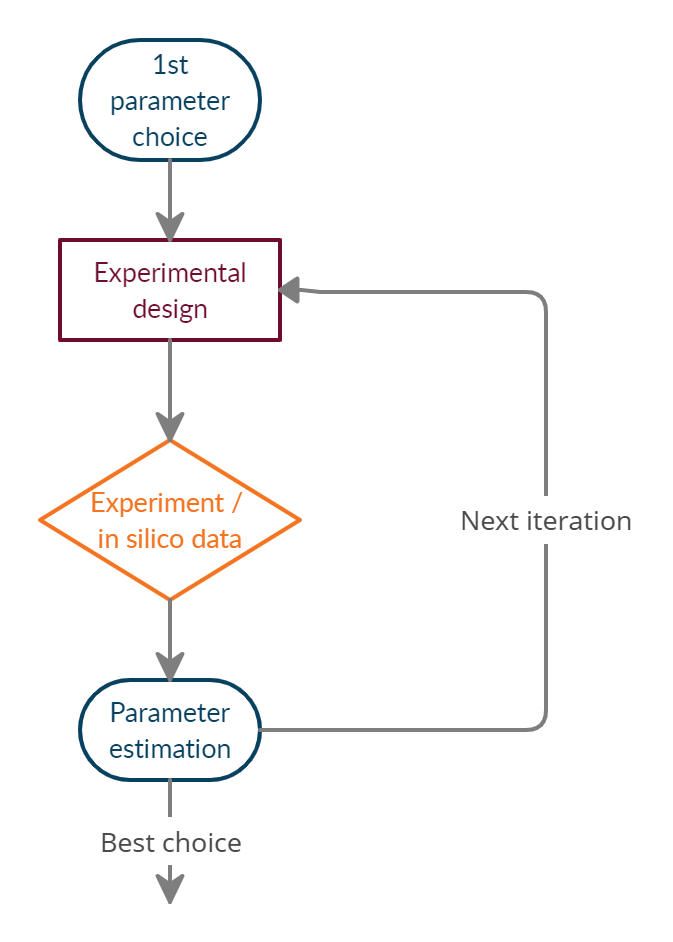
\includegraphics[scale=0.25]{Figures/scheme.png}
    \caption{{\footnotesize The workflow of the iterative process of model optimization for parameter estimation.}}
    \label{fig:expdesign_scheme}
\end{figure}
In the beginning, we would like to briefly describe the whole iterative process of model building (see Fig. \ref{fig:expdesign_scheme}).
Firstly, based on the literature review or prior data from pilot experiments, the first parameter estimation of the chosen model structure should be done.
The obtained values can be applied to propose the first optimal experimental design accounting for different constraints, e.g., the lab limitations, human resources, etc. 
Depending on availability, either real or numerical experiments should be conducted based on this design to gather measurement or in-silico data. 
This new data can be used for the new parameter estimations values with corresponding uncertainties.
After this, using new parameter values, the process can be repeated several times to increase the precision of the parameter estimates till the desired accuracy is achieved.
%
%
%
% ########################################################################
% ########################################################################
\section*{Materials and Methods}
This tutorial expects a working installation of the popular scripting language Python $\geq3.7$~\cite{rossumPythonLanguageReference2010}.
For installation instructions, please refer to the website \href{https://www.python.org/downloads/}{python.org}.
We also expect users, to be able to write, execute and display output of scripts.
This tutorial can also be followed using jupyter notebooks.

We have developed \mintinline[bgcolor=white,style=emacs]{bash}{FisInMa}, which is a set of tools to calculate the Sensitivity and Fischer Information Matrix and do parameter space exploration in order to find optimal results.
Users can obtain it by installing \mintinline[bgcolor=white,style=emacs]{bash}{FisInMa} from \href{https://pypi.org/project/FisInMa/0.0.1/}{pypi.org}.
The python website has guides for installing packages \href{https://packaging.python.org/en/latest/tutorials/installing-packages/}{packaging.python.org/}.
Most Unix-Based systems (eg. GNU/Linux) and Mac-OS can use \mintinline[bgcolor=white,style=emacs]{bash}{pip}
\begin{minted}[bgcolor=white]{bash}
pip install FisInMa
\end{minted}
or \mintinline[bgcolor=white,style=emacs]{bash}{conda} to install the desired package.
\begin{minted}[bgcolor=white]{bash}
conda install FisInMa
\end{minted}
The \href{https://spatial-systems-biology-freiburg.github.io/FisInMa/}{Documentation} of the package is continuously updated.
After the installation of the package is complete, we open a file with a text editor of choice and simply start writing code.
We begin by writing a so-called she-bang which is responsible to signalize that this file is to be executed with python.
Afterwards, we import the needed packages.
\begin{code}[h]
    \begin{minted}[firstnumber=1]{python}
    #!/usr/bin/env python3

    import numpy as np
    from FisInMa import *
    \end{minted}
    \caption{Import statements to use FisInMa}
    \label{code:import_statements}
    % TODO make this FisInMa into a link
\end{code}
This will serve as the starting point for our script.
In the following, we will append more code to it and utilize the methods developed in FisInMa~\cite{}.% TODO add citation which points to github repository
If line numbers are missing, these should be filled by blank lines for better readability.
%
%
% ########################################################################
\subsection*{Model Formulation}
\subsubsection*{Theory}
The first important step a reader should do to conduct their Experimental Design is to define a model structure.
In this chapter, we restrict ourselves to a quite popular case in Predictive Microbiology and assume that biological system is described by a system of \aclp{ode}
\begin{equation}
    \begin{cases}
    \dot \mbx (t) = f(t, \mbx, \mbu, \mbp) \\
    \mbx (t_0) = \mbx_0
    \label{eq:ode_general}
    \end{cases}.
\end{equation}
Here $\mbx = (x_1, x_2, ..., x_n)$ is a vector of state variables of the system with initial condition $\mbx_0$, $t$ is a time, $\mbu$ is a vector of an externally controlled inputs and $\mbp$ are the parameters of the system.
The parameters of the system are unknown and can be estimated from the data.
Another important choice to be done is to define the observables of the system $\mby$, which quantities and at which times $t_i$ should be measured.
\begin{equation}
    \mby (t_i) = g(t_i, \mbx (t_i), \mbu, \mbp) + \epsilon (t_i),
    \label{eq:observ_general}
\end{equation}
where the function $g$ describes the model output, and $\epsilon$ is the measurement noise. 
The observational noise is often assumed to be an independently distributed Gaussian noise with zero mean and variance $\sigma_i^2$: $\epsilon (t_i) \sim N(0, \sigma_i^2)$.

Here, to demonstrate how Experimental Design works, we will refer to a widely used Baranyi and Roberts model (1994) that can be used, for example, to describe bacteria growth.
The model is introduced by two state variables $\mbx = (x_1, x_2)$, where $x_1(t)$ denotes the cell concentration of a bacterial population at the time $t$ and $x_2(t)$ defines a physiological state of the cells, the process of adjustment (lag-phase):
\begin{equation}
    \begin{cases}
        \dot x_1(t) = \frac{x_2(t)}{x_2(t) + 1} \mu^\text{max} \big(1 - \frac{x_1(t)}{x_1^\text{max}}\big) x(t)  = f_1 \\
        \dot x_2(t) = \mu^\text{max}  x_2(t) = f_2
    \end{cases}.
    \label{eq:ode_BaranyiRoberts}
\end{equation}
Here $\mu^\text{max}$ determines the maximum growth rate, and $x_1^\text{max}$ is the bacteria concentration at the saturation. 
To account for the influence of the temperature on the activity of the model, we will use the 'square root' or Ratkowsky-type model for the maximum growth rate
\begin{equation}
    \sqrt{\mu^\text{max}} = b (T - T_\text{min}),
    \label{eq:RatkowskyModel}
\end{equation} 
where $b$ is the regression coefficient, and $T_\text{min}$ is the minimum temperature at which the growth can occur.
As an observable, it is pretty common to measure the bacteria count $x_1$ or the logarithm of this value. 
For simplicity, we would consider the prior case $y(t_i) = x_1(t_i)$.
The system is fully defined by equations (\ref{eq:ode_BaranyiRoberts}), (\ref{eq:RatkowskyModel}).
Here $x_1^\text{max}, b, T_\text{min}$ are the parameters that we estimate using observational data $y$ at measurement times $t_i$, and temperature $T$ is an input of the system.
Based on this model, we would like to optimize the choice of measurement times as well as temperatures (inputs) of the system to find the \acl{oed}.
%
% ########################################################################
\subsubsection*{Code}
In order to be able to solve these equations numerically, we first need to define the \ac{ode} system in python.
As was explained in the previous sections, this system consists of the equation (\ref{eq:ode_general}) with initial values $t_0,x_0$.
Next, we need to define all numerical values present in the system.
We distinguish between time points $t_i$ at which the result of the \ac{ode} is evaluated, inputs $u$, which alter the behaviour of our system (for example temperature, humidity, etc.), parameters $p$, which are the quantities that we want to measure and other arguments which might be needed to solve the \ac{ode}.
Table \ref{tab:fsm-variables} summarizes them and gives representations in the code.
In the following, we will gradually explain how to specify all variables needed by using the example of the Baranyi-Roberts Model as given in equations (\ref{eq:ode_BaranyiRoberts}).
\begin{table}[H]
    \centering
    \begin{tabular}{ccccc}
        \specialrule{.1em}{.01em}{.05em}
        Description & Formula & Code \\[1ex]
        \toprule \vspace{1mm} 
        ODE & $f$                       & \mintinline[bgcolor=white,style=emacs]{python}{def ode_fun(t, x, u, p, ode_args):} \\
            & $\partial f / \partial x$ & \mintinline[bgcolor=white,style=emacs]{python}{def ode_dfdx(t, x, u, p, ode_args):} \\[0.5ex]
            & $\partial f / \partial p$ & \mintinline[bgcolor=white,style=emacs]{python}{def ode_dfdp(t, x, u, p, ode_args):} \\[0.5ex]
        \midrule
        Observable  & $g$                       &  \mintinline[bgcolor=white,style=emacs]{python}{def obs_fun(t, x, u, p, ode_args)}\\[0.5ex]
        (optional)  & $\partial g / \partial x$ &  \mintinline[bgcolor=white,style=emacs]{python}{def obs_dgdx(t, x, u, p, ode_args)}\\[0.5ex]
                    & $\partial g / \partial p$ &  \mintinline[bgcolor=white,style=emacs]{python}{def obs_dgdp(t, x, u, p, ode_args)}\\[0.5ex]
        \midrule
        Initial value   & $x_0$ & \mintinline[bgcolor=white,style=emacs]{python}{x0}\\[0.5ex]
        Initial time    & $t_0$ & \mintinline[bgcolor=white,style=emacs]{python}{t0}\\[0.5ex]
        Time points     & $t_i$ & \mintinline[bgcolor=white,style=emacs]{python}{t}\\[0.5ex]
        Inputs          & $u$   & \mintinline[bgcolor=white,style=emacs]{python}{u}\\[0.5ex]
        Parameters      & $p$   & \mintinline[bgcolor=white,style=emacs]{python}{p}\\[0.5ex]
        Other arguments &       & \mintinline[bgcolor=white,style=emacs]{python}{ode_args}\\[0.5ex]
        \bottomrule
    \end{tabular}
    \caption{Summary of user-defined functions and variables.}
\label{tab:fsm-variables}
\end{table}
\paragraph{Defining the \acs{ode}} First, we must define a few functions in python.
The first function will be the right-hand side of equation (\ref{eq:ode_general}), which means for the Baranyi-Roberts model, we can simply copy equation (\ref{eq:ode_BaranyiRoberts}) into a function.
The complete function can be seen in Figure \ref{code:code_baranyi_roberts_ode_fun}.
We explain the individual steps to recreate this function.
The order of required function arguments is fixed by the signature
\mintinline[bgcolor=white,style=emacs]{python}{def ode_fun(t, x, u, P, ode_args)} whereas the function name can be given freely and should represent the model in which we are interested.
Since the state variable \mintinline[bgcolor=white,style=emacs]{python}{x} is a $2D$ vector, we can use python notation to unpack this vector to two individual variables
\mintinline[bgcolor=white,style=emacs]{python}{(x1, x2) = x}.
In general, we can have multiple inputs, which is why \mintinline[bgcolor=white,style=emacs]{python}{u} is also a vector and needs to be unpacked in order to use it directly \mintinline[bgcolor=white,style=emacs]{python}{(Temp,) = u}.
The same procedure is carried out for the parameters \mintinline[bgcolor=white,style=emacs]{python}{(x_max, b, Temp_min) = p}.
We can now do some mathematical calculations of intermediate values that we will use in the final output.
In our example, we calculate the maximum growth rate via \mintinline[bgcolor=white,style=emacs]{python}{mu_max = b**2 * (Temp - Temp_min)**2}.
The result of equation \ref{eq:ode_BaranyiRoberts} is then given by \mintinline[bgcolor=white,style=emacs]{python}{mu_max * (x2/(x2 + 1)) * (1 - x1/x_max) * x1} and 
\mintinline[bgcolor=white,style=emacs]{python}{mu_max * x2} respectively.
We store these results in a list (denoted by \mintinline[bgcolor=white,style=emacs]{python}{[ ... ]}) and return it.
\begin{code}[h]
    \begin{minted}[firstnumber=6]{python}
    def baranyi_roberts_ode(t, x, u, p, ode_args):
        (x1, x2) = x
        (Temp, ) = u
        (x_max, b, Temp_min) = p
        # Define the maximum growth rate
        mu_max = b**2 * (Temp - Temp_min)**2
        return [
            mu_max * (x2/(x2 + 1)) * (1 - x1/x_max) * x1,
            mu_max * x2
        ]
    \end{minted}
    \caption{Definition of the Baranyi-Roberts \ac{ode} model.}
    \label{code:code_baranyi_roberts_ode_fun}
\end{code}
%
% ########################################################################
\subsection*{Parameter Estimation}
One of the requirements for conducting an Experimental Design is a provision of parameter values by a user.
Due to this, after the model was defined, the first parameter values should be chosen from the literature or estimated from previously gathered experimental data by maximizing the likelihood function.
By definition, the likelihood function $L(\mbp)$ is the probability of observing a data $\mby$ in case of a certain parameters $\mbp$: $L(\mbp) = p(\mby|\mbp)$.
With the assumption of the Gaussian white measurement noise with zero mean and variance $\sigma_i^2$: $\epsilon(t_i) \sim N(0, \sigma_i^2)$, it is convenient to maximize the logarithm of the likelihood function (log-likelihood) instead.
This is likewise simply minimizing the sum of the squared difference between the measured data and model output:
\begin{equation}
    \ln L(\mbp) \propto - \sum_{i}\frac{ \big(\mathbf{g}^{i}(\mbp) - \mby^{i}\big)^2}{2 \sigma_{i}^2}.
    \label{eq:likelihood_Gaussian}
\end{equation}
Here $\mby^{i}$ is the $i$-th value of observational data, and $\mathbf{g}^{i}(\mbp)$ is a corresponding to it model output.
%
% ########################################################################
\subsection*{Experimental Design}
And finally, the reader can now proceed directly to the Experimental Design.
The methods of the Experimental Design imply maximizing the objective function calculated using one of the properties of the \ac{fim}.
According to the so-called 'Cramer-Rao inequality', the Fisher information is inversely proportional to the minimal squared estimation error \cite{friedenExploratoryData2010}. 
So its maximization actually leads to minimization of the uncertainty of the parameter estimates.
We are going to explain one of the ways to calculate this so-called \acl{fim} for mentioned above \acp{ode} system (\ref{eq:ode_general}) and the observable function (\ref{eq:observ_general}).
%
% ########################################################################
\subsubsection*{Sensitivity Calculation}
Assume that functions $f$ and $g$ are differentiable functions with respect to the state varibles $\mbx$ and parameters $\mbp$.
The first step is to calculate local sensitivities $s^x_{ij} = (\mathrm{d} x_i / \mathrm{d} p_j )$.
To do this, we need to solve the following system of the \acp{ode}:
\begin{equation}
    \begin{cases}
    \dot x_i (t) = f_i(t, \mbx, \mbu, \mbp)\\
    \dot s^x_{ij} = \sum_k \frac{\partial f_i}{\partial x_k} s^x_{kj} + \frac{\partial f_i}{\partial p_j}
    \end{cases}.
\label{eq:ode_and_sensitiv}
\end{equation} 
The \ac{fim} is composed only with those sensitivity coefficients that correspond to the observables.
That means that the next step is to calculate $(\mathrm{d} y_i / \mathrm{d} p_j) = s_{ij}$ at a certain times $t_m$ and input $u_n$ using the solutions of $s^x_{ij}$:
\begin{equation}
    s_{ij} (t_m, u_n) = \sum_k \frac{\partial g_i}{\partial x_k}\bigg|_{t_m, u_n} s_{kj}^x (t_m, u_n) + \frac{\partial g_i}{\partial p_j}\bigg|_{t_m, u_n}.
\label{eq:observ_sensitivities}
\end{equation}

In the case of the parameters with different dimensionalities and values of different orders of magnitude, it makes sense to use the relative sensitivities instead
\begin{equation}
    \tilde{s}_{ij} (t_m, u_n) = \frac{\mathrm{d} y_i}{\mathrm{d} p_j} \frac{p_j}{y_i}\bigg|_{t_m, u_n}
\label{eq:relat_sensitivities}
\end{equation}
to improve not the absolute but the relative accuracy of the parameter estimates.

These sensitivities should be arranged to be elements of the sensitivity matrix.
For example, in case of two observables $\mby = (y_1, y_2)$, two different inputs $\mbu = (u_1, u_2)$, $N$ different time and $N_p$ parameters, sensitivity matrix will look in the following way:
\begin{equation}
    S = 
\begin{bmatrix}
s_{11} (t_1, u_1) & ... & s_{1 N_p}(t_1, u_1) \\
\vdots  &   & \vdots  \\
s_{11} (t_{N}, u_1) & ... & s_{1 N_p} (t_{N}, u_1)\\
s_{11} (t_1, u_2) & ... & s_{1 N_p}(t_1, u_2) \\
\vdots  &   & \vdots  \\
s_{11} (t_N, u_2) & ... & s_{1 N_p} (t_N, u_2)\\

s_{21} (t_1, u_1) & ... & s_{2 N_p}(t_1, u_1) \\
\vdots  &   & \vdots  \\
s_{21} (t_{N}, u_1) & ... & s_{2 N_p} (t_{N}, u_1)\\
s_{21} (t_1, u_2) & ... & s_{2 N_p}(t_1, u_2) \\
\vdots  &   & \vdots  \\
s_{21} (t_N, u_2) & ... & s_{2 N_p} (t_N, u_2)
\end{bmatrix}
\label{eq:sens_matrix}
\end{equation}

This matrix we will use to directly calculate the \ac{fim} via equation:
\begin{equation}
    F = S^T Q^{-1} S,
\end{equation}
where $Q$ is the covariance matrix of measurement error.
If all measurements are considered independent, then only diagonal elements of the matrix are non-zero: 
\begin{equation}
    Q = 
\begin{pmatrix}
    \sigma_{1}^2(t_1, u_1) & 0                      & 0                      & \dots  & 0                     \\
    0                      & \sigma_{1}^2(t_2, u_1) & 0                      & \dots  & 0                     \\
    0                      & 0                      & \sigma_{1}^2(t_1, u_2) & \dots  & 0                     \\
    \vdots                 & \vdots                 & \vdots                 & \ddots & \vdots                \\
    0                      & 0                      & 0                      & \dots  & \sigma_{2}^2(t_N, u_2)
\end{pmatrix}.
\label{eq:covar_matrix}
\end{equation}
Here $\sigma_{i}^2 (t_m, u_n)$ is the variance obtained from the measurement of observable $y_i$ at time point $t_m$ with input $u_n$.
The variance value can be either calculated from the real data or approximated by some error model.
For example, one may consider that the error contribution consists of an absolute part that stays constant and a relative part that is proportional to observable value.
Then the diagonal elements of the covariance matrix take form:
\begin{equation}
    \sigma_{i}^2 (t_m, u_n) = \gamma_\text{abs} + \gamma_\text{rel} \cdot y_i(t_m, u_n),
\end{equation}
where $\gamma_\text{abs}$ and $\gamma_\text{rel}$ are the coefficients determining the absolute and the relative error contribution, relatively.
In case of relative sensitivities $\tilde{s}_{ij} (t_m, u_n)$, it makes sence to talk also about relative covariance matrix.
The elements of such a relative matrix can be calculated as:
\begin{equation}
    \tilde{\sigma}_{i}^2 (t_m, u_n) = \frac{\sigma_{i}^2 (t_m, u_n)}{y^2_i(t_m, u_n)}.
\end{equation} 
%
% ########################################################################
\subsection*{Numerical Sensitivity Calculation}
To calculate the sensitivities numerically as just explained, we additionally need to supply the derivatives of $f$ with respect to the parameters and state variables used in equation (\ref{eq:observ_sensitivities}).
Thus, we need to define functions for these derivatives as well.
Firstly, we calculate the mathematical derivatives $\partial f_i/\partial p_j$ and $\partial f_i/\partial x_j$ and then implement the functions.
In our case, the first component of the Baranyi-Roberts model reads
\begin{equation}
    \dot x_1(t) = f_1(t, x) = \mu^\text{max} \frac{x_2(t)}{x_2(t) + 1} \left(1 - \frac{x_1(t)}{x_1^\text{max}}\right) x(t)
\end{equation}
where $\sqrt{\mu^\text{max}}=b(T-T_\text{min})$.
Since the later quantitiy $\mu^\text{max}$ depends on $b$ and $T_\text{min}$, we also need to take into account their derivatives.
\begin{alignat}{4}
    \frac{\partial\mu^\text{max}}{\partial p_1} &= 0\\
    \frac{\partial\mu^\text{max}}{\partial p_2} &= 2b(T-T_\text{min})^2 &= \frac{2\mu^\text{max}}{b}\\
    \frac{\partial\mu^\text{max}}{\partial p_3} &= -2b^2(T-T_\text{min}) &= \frac{2\mu^\text{max}}{T-T_\text{min}}
\end{alignat}
Thus the derivatives of the first component of $f$ with respect to $p_1=x_{max}$, $p_2=b$ and $p_3=T_\text{min}$ are
\begin{alignat}{7}
    \frac{\partial f_1}{\partial p_1}(t) &= - \mu^\text{max} &&\frac{x_2(t)}{x_2(t) + 1} &\frac{x_1(t)}{\left(x_1^\text{max}\right)^2} &&x(t)\\
    \frac{\partial f_1}{\partial p_2}(t) &= \frac{2\mu^\text{max}}{b} &&\frac{x_2(t)}{x_2(t) + 1} &\left(1 - \frac{x_1(t)}{x_1^\text{max}}\right) &&x(t)\\
    \frac{\partial f_1}{\partial p_3}(t) &= \frac{2\mu^\text{max}}{T-T_\text{min}} &&\frac{x_2(t)}{x_2(t) + 1} &\left(1 - \frac{x_1(t)}{x_1^\text{max}}\right) &&x(t)
\end{alignat}
respectively.
Similarly, the derivatives $\partial f/\partial x_i$ are
\begin{alignat}{7}
    % TODO
    \frac{\partial f_1}{\partial x_1}(t) &= \mu^\text{max} &\frac{x_2(t)}{x_2(t) + 1} && \left(-\frac{1}{x_1^\text{max}}\right) &&x(t)\\
    \frac{\partial f_1}{\partial x_2}(t) &= \mu^\text{max} &\left(\frac{1}{x_2(t) + 1} - \frac{x_2(t)}{(x_2(t) + 1)^2}\right) && \left(1 - \frac{x_1(t)}{x_1^\text{max}}\right) &&x(t)
    % TODO
\end{alignat}
The readers are encouraged to calculate the components $\partial f_2/\partial p_i$ and $\partial f_2/\partial x_i$ by themselves since these are still missing for a complete set.
Assuming, we carried out the necessary mathematical derivation, the implemented functions in python can be seen in Figure~\ref{code:code_baranyi_roberts_ode_fun_derivatives}.
\begin{code}[H]
    \begin{minted}[firstnumber=20]{python}
    def ode_dfdp(t, x, u, p, ode_args):
        (x1, x2) = x
        (Temp, ) = u
        (x_max, b, Temp_min) = p
        mu_max = b**2 * (Temp - Temp_min)**2
        return [
            [
                mu_max * (x2/(x2 + 1)) * (x1/x_max)**2,
                2 * b * (Temp - Temp_min)**2 * (x2/(x2 + 1))
                    * (1 - x1/x_max)*x1,
                -2 * b**2 * (Temp - Temp_min) * (x2/(x2 + 1))
                    * (1 - x1/x_max)*x1
            ],
            [
                0,
                2 * b * (Temp - Temp_min)**2 * x2,
                2 * b**2 * (Temp - Temp_min) * x2
            ] 
        ]

    def ode_dfdx(t, x, u, p, ode_args):
        (x1, x2) = x
        (Temp, ) = u
        (x_max, b, Temp_min) = p
        mu_max = b**2 * (Temp - Temp_min)**2
        return [
            [
                mu_max * (x2/(x2 + 1)) * (1 - 2*x1/x_max),
                mu_max * 1/(x2 + 1)**2 * (1 - x1/x_max)*x1
            ], 
            [
                0,
                mu_max
            ]
        ]
    \end{minted}
    \caption{Derivatives of the function $f$ of the Baranyi-Roberts model \ac{ode}.}
    \label{code:code_baranyi_roberts_ode_fun_derivatives}
\end{code}
%
% ########################################################################
\subsection*{Define numerical values}
Now that we have defined the structure of our \ac{ode}, we can begin to specify numerical values.
It is good practice, to gather such definitions in the \mintinline[bgcolor=white,style=emacs]{python}{__main__} method of our program as was done in Figure~\ref{code:code_write_main_function_start}.
We start by defining the parameters (line 59) of our \ac{ode} and afterwards the initial values of the \ac{ode} (line 62).
Next, we want to tell the program to choose the best possible time points in the interval $t_i\in\left[t_\text{low},t_\text{high}\right]$ in the optimization routine later on.
To do this, we write the times as a dictionary with entries \mintinline[bgcolor=white,style=emacs]{python}{{"lb":t_low, "ub":t_high, "n":n_times}} where \mintinline[bgcolor=white,style=emacs]{python}{n_times} is the number of time points which we want to sample (line 65).
In contrast, if we wanted to specify explicit values for the time points, we would have needed to supply a list of time values or a \mintinline[bgcolor=white,style=emacs]{python}{np.ndarray} directly.
One can see this aproach when we define the inputs in line 70.
Here, we supply a \mintinline[bgcolor=white,style=emacs]{python}{np.ndarray} with explicit values, thus fixing them for the optimization routine.
\begin{code}[h]
    \begin{minted}[firstnumber=57]{python}
    if __name__ == "__main__":
        # Define parameters
        p = (np.exp(21.1), 0.038, 2)

        # Define initial conditions
        x0 = np.array([np.exp(2.36), 1 / (np.exp(2.66)-1)])

        # Define interval and number of sampling points for times
        times = {"lb":0.0, "ub":1500.0, "n":4}

        # Define explicit temperature points
        Temp_low = 4.0
        Temp_high = 8.0
        n_Temp = 3

        # Summarize all input definitions in list (only temperatures)
        inputs = [
            np.linspace(Temp_low, Temp_high, n_Temp)
        ]
    \end{minted}
    \caption{The main function contains the actual values for our model definition.}
    \label{code:code_write_main_function_start}
\end{code}
\subsubsection*{Defining Explicit Values and Sampling}
The difference between choosing explicit values and specifying a sampling range may be subtle to see at first glance, but in turn allows to very easily switch between fixed values and sampling.
For example, suppose we wanted to also sample temperature points, which means we let the optimization algorithm pick the optimal temperature points such that the information gathered from the system is maximized.
Then the difference between explicit values for the temperatures and sampled ones can be seen in code sample~\ref{code:difference_explicit_sampling}.\newline
\begin{code}[h]
    \begin{minted}[linenos=false]{python}
    # This will choose values explicitly
    inputs = [
        np.linspace(Temp_low, Temp_high, n_Temp)
    ]
    # >>> inputs
    # [array([4., 6., 8.])]


    # This will sample in the interval
    inputs = [
        {"lb":Temp_low, "ub":Temp_high, "n":n_Temp}
    ]
    # >>> inputs
    # [{'lb': 4.0, 'ub': 8.0, 'n': 3}]


    \end{minted}
    \caption{Difference between choosing explicit values and sampling over a given interval.}
    \label{code:difference_explicit_sampling}
\end{code}%
This distinction can be done for individual inputs as well.
Suppose, we have a system with temperatures and humidity as input variables.
We could decide to pick the best temperature points, but fix the humidity explicitly.
This can be beneficial, if one of the variables can be controlled (i.e. temperature in the lab) but the other is more difficult to fix (i.e. humidity).
In our code, we simply would mix explicit and sampled definitions for individual inputs (see code sample~\ref{code:mix_sampling_explicit}).
\begin{code}[h]
    \begin{minted}[linenos=false]{python}
        inputs = [
            # These values will be sampled
            {"lb":Temp_low, "ub":Temp_high, "n":n_Temp},
            # These are fixed
            np.array([0.4, 0.45, 0.5, 0.55])
        ]
    \end{minted}
    \caption{Mixing of explicit and sampling for inputs.}
    \label{code:mix_sampling_explicit}
\end{code}
%
% ########################################################################
\subsection*{Define Model}
After we have decided on the numerical values for our model, we need to supply them to the program.
The \mintinline[bgcolor=white,style=emacs]{python}{FisherModel} class serves as the entry point.
Here, we simply supply every previously made definition of variables and methods.
When using the syntax as shown in code sample~\ref{code:model_definition}, the order of arguments does not matter.
However, when only using \mintinline[bgcolor=white,style=emacs]{python}{FisherModel(x0, 0.0, ...)}, please pay attention to the order of arguments.
\begin{code}[H]
    \begin{minted}[autogobble=false,firstnumber=77]{python}
    # Create the FisherModel which serves as the entry point
    #  for the solving and optimization algorithms
    fsm = FisherModel(
        ode_x0=x0,
        ode_t0=0.0,
        ode_fun=baranyi_roberts_ode,
        ode_dfdx=ode_dfdx,
        ode_dfdp=ode_dfdp,
        ode_initial=x0,
        times=times,
        inputs=inputs,
        parameters=p
    )
    \end{minted}
    \caption{Define the full model.}
    \label{code:model_definition}
\end{code}
There are some optional arguments which can be set if desired ...
% TODO
% TODO
For a full list of optional arguments, we refer to the \href{https://spatial-systems-biology-freiburg.github.io/FisInMa/}{documentation} of the package.
%
% ########################################################################
\subsubsection*{Identifiability}
Here, before proceeding with optimization, the reader should take the time and check if the system is identifiable, meaning that if it is possible to obtain the unique solution from the optimization. 
The non-identifiability can be due to the wrong choice of the model structure or observable (structural) or the incorrect choice of gathered data (practical).
The quick and easy way to check the system on structural non-identifiability is to calculate the rank of the sensitivity matrix.
For an identifiable system, it should coincide with the number of estimated parameters.
If this condition is satisfied, we can continue with optimization.
%
% ########################################################################
\subsubsection*{Optimality Criteria}
Different optimality criteria choose to maximize different objectives.
The effects of these objectives on the parameter space can vary so the reader can choose the most suitable one. 
Some of the most popular criteria we would like to mention:
\begin{itemize}
    \item \textbf{D-optimality criterion} maximizes the determinant $\det (F)$ of the \ac{fim}. 
    In parameter space it means that we minimize the volume of so-called confidence region (see Fig. \ref{fig:opt_criteria}), or geometrical mean of the errors.
    The confidence region at a confidence level of $\alpha$ can be interpreted as there is a $\alpha \cdot 100 \%$ chance that the best parameter fit will belong to this area in case of repeating the experiment and estimations multiple times.
    It is usually presented as a confidence ellipsoid.
    D-optimality is the most widely used criterion and is suitable even if the parameters have different dimensionalities.
    
    \item \textbf{E-optimality criterion} concentrates on maximizing the minimal eigenvalue $\lambda_{\min}$ of the \ac{fim}, which is the same as reducing only the largest estimation error.
    
    \item \textbf{A-optimality criterion} takes into account the sum of all eigenvalues $\sum_i \lambda_i$
    That can be interpreted as minimizing the algebrasic mean of all errors.
    
    \item \textbf{Modified E-optimality criterion} is also rather promising method that maximizes the ratio between the minimal and maximal eigenvalue $\lambda_{\min} / \lambda_{\max}$.

\end{itemize}
Each of the criteria has its pros and cons so the reader can take a closer look at the various properties of these criteria, for instance, in Franceschini's and Macchietto's paper \cite{franceschiniModelbasedDesignExperiments2008}.
For a better understanding, we can geometrically interpret the criteria using the confidence region shown in Fig. \ref{fig:opt_criteria}.
\begin{figure}[H]
    \centering
    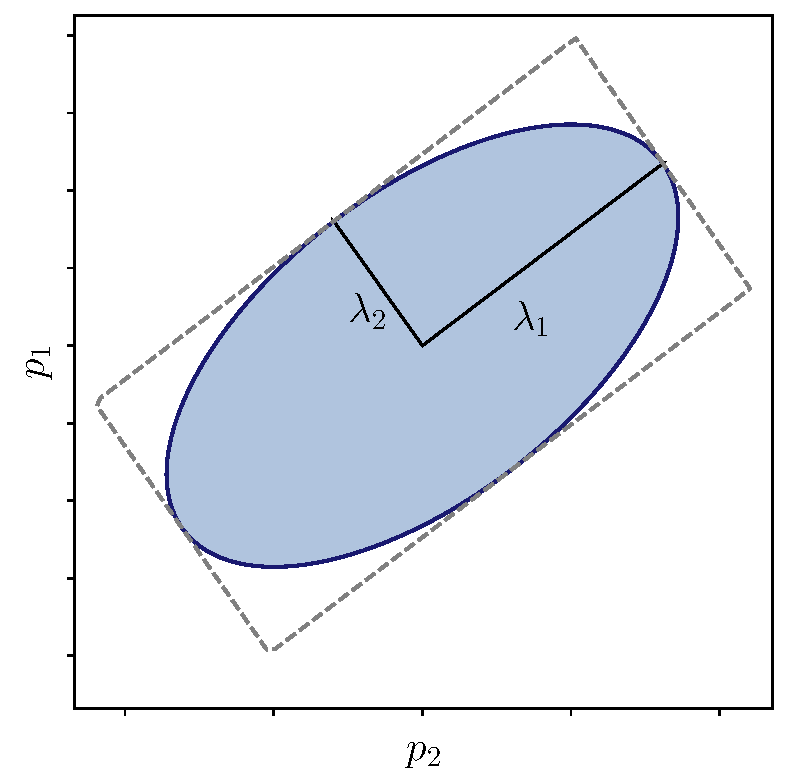
\includegraphics[scale=0.6]{Figures/optimality_criteria.pdf}
    \caption{{\footnotesize The confidence ellipsoid projection to the ($p_1$, $p_2$) parameter space. 
    The ellipsoid shows the geometrical meaning of the optimality criteria. 
    The center of the ellipsoid represents the estimated parameter values.
    The radii are the uncertainties of the estimates associated with different eigenvalues of the \ac{fim} $\lambda_1$, $\lambda_2$ ($\lambda_1 < \lambda_2$).
    The D-optimality aims to minimize the volume of the ellipsoid, the E-optimality minimizes the largest radius, A-optimality minimizes the perimeter of the rectangle that encloses the ellipse (dashed gray line), and, finally,  Modified E-optimality tends to make the ellipse as spherical as possible.}}
    \label{fig:opt_criteria}
\end{figure}
%
% ########################################################################
\subsubsection*{Optimization}
The described above technique can be used to calculate the objective function (Fisher optimality criterion) for a certain experimental scheme.
Finding the Experimental Design that corresponds to the global maximum of the objective is a special case of optimal control problem.
This problem is widely studied, and multiple numerical solution algorithms for both local and global optimization were introduced.
In the suggested toolbox, three methods were implemented: differential evolution, basin-hopping, and brute force.

Quite good results can be achieved by the \ac{de} algorithm developed by Storn and Price (1996) \cite{stornDifferentialEvolutionSimple1997}.
It is one of the stochastic global optimization methods that show rather good results for nonlinear dynamic problems.
Such approaches help to greatly improve computational times but sacrifice is that one cannot be sure that the absolute optimum is reached.
Firstly, the initial population of candidate solutions is randomly chosen from the region of available values.
In our case, these solutions are the vectors of all optimized values (times and inputs) for one Experimental Design.
Then each solution mutates by mixing with other candidates.
To a chosen one solution from the initial population $D_0$, we add a weighted difference between two other random solutions from the same set $(D_\text{rand1} - D_\text{rand2})$.
This process is called mutation and a new vector $D_m$ is obtained.
The next step is to construct a new trial solution.
This is done by randomly choosing the elements of this vector either from the initial $D_0$ or the mutated $D_m$ solutions.
For each new element of trial vector, from the segment [0, 1) the number should be randomly picked and compared to the so-called recombination constant.
If this number is less than a constant, then the new solution element is chosen from mutated vector $D_m$, otherwise from $D_0$.
So, in general, the degree of mutation can be controlled by changing this recombination constant.
When the trial candidate is built, it is compared to initial solution $D_0$, and the best of them is chosen for the next generation.
This operation is repeated for every solution candidate of the initial population, and the new population generation can be formed.
The process of population mutation is repeated till the desired accuracy is achieved.
This method is rather simple, straightforward, does not require the gradient calculation and is able to be parallelized.

The second method is the basin-hopping developed by David Wales and Jonathan Doye \cite{walesGlobalOptimizationBasinHopping1997}. 
It combines the Monte-Carlo and local optimization and works as follows. 
The classic Monte-Carlo algorithm implies that the values of the optimized vector are perturbed and are either accepted or rejected.
However, in this modified strategy, after perturbation, the vector is additionally subjected to local minimization.
And only after this procedure the move is accepted according to the Metropolis criterion.


And lastly, the brute force method was implemented as well.
It is a grid search algorithm calculating the objective function value at each point of a multidimensional grid in a chosen region.
The advantage of this algorithm is that we can be sure that the global minimum is achieved while all possibilities are checked.
However, this technique is rather slow and inefficient.
Even though the discretization and reduction of the whole number of possible values can improve the performance, the computational time allows optimization only for a small number of optimization times or inputs.

Some other optimization methods for the optimal control problem the reader can find, for example, in the papers of Banga \etal \cite{BANGA2005407, bangaImprovingFoodProcessing2003}.
%
% ########################################################################
\subsubsection*{Optimization Code}
The usage of these optimization methods is greatly simplified in our approach.
\begin{minted}[linenos=false]{python}
fsr = find_optimal(fsm)
\end{minted}
However, we retain their full functionality.
Any optmization argument that could be specified to any of the aforementioned routines, can be specified here and will be applied to the optimization.
\begin{minted}[autogobble=false,firstnumber=98]{python}
    fsr = find_optimal(
        # Required argument: The model to optimize
        fsm,
        # Our custom options
        criterion=fisher_determinant,
        relative_sensitivities=True,
        # Options from scipy.optimize.differential_evolution
        recombination=0.7,
        mutation=(0.1, 0.8),
        workers=-1,
        popsize=10,
        polish=False,
    )
\end{minted}
A full list of optional arguments can be seen in the \href{https://docs.scipy.org/doc/scipy/reference/optimize.html#global-optimization}{scipy documentation}~\cite{virtanenSciPyFundamentalAlgorithms2020}.
In addition, there are some interesting optimization options such as the optional arguments \mintinline[bgcolor=white,style=emacs]{python}{relative_sensitivities,criterion}, which are responsible for using relative sensitivities $\tfrac{dy}{dp}\tfrac{p}{y}$ and specifying the optimality criterion as explained in the previous section.
Please view the \href{https://spatial-systems-biology-freiburg.github.io/FisInMa/}{full documentation} for explanation.
The resulting class is a \mintinline[bgcolor=white,style=emacs]{python}{FisherResult} containing all definitions, current values and information on the optimization process.
%
% ########################################################################
\subsubsection*{Plotting, Json, etc.}
Our package also provides the option to save results as a Json file and automatically plot results for the ode solutions, observables and sensitivities.

\begin{minted}[autogobble=false,firstnumber=92]{python}
    plot_all_observables(fsr)
    plot_all_sensitivities(fsr)
    json_dump(fsr, "baranyi.json")
\end{minted}
%
%
%
% ########################################################################
% ########################################################################
\section*{Conclusion}
Summarizing the above tutorial, we would like to present the resulting output of our package.
For this, consider the following example.
One wants to study a real-life system and describe it with the Baranyi and Roberts model (\ref{eq:ode_BaranyiRoberts},\ref{eq:RatkowskyModel}).
However, experimenters claim that they can conduct only one experimental series for one constant temperature value and measure the first component of the state variable vector $y = x_1$.
The refrigerating chambers available in operation can maintain the temperature only in the range from 3 to 12 degrees.
After some literature search, it was found that for the similar systems the approximate parameter values are $x_1^\text{max}=10^8$, $b=0.2$, $T_\text{min}=1.0$,
and the initial conditions for the system of \acp{ode} are about $x_1(0) = 10^3$, $x_2(0)=0.01$.
Moreover, all the measurements contain constant error $\gamma_\text{abs}=0.3$ and in addition an error term proportional to observable value $\gamma_\text{rel}=0.1$.
The task is to propose at which temperature and times it will be better to measure from the modeling point of view.

To solve this problem, we performed the Experimental Design using the D-optimality criterion, relative sensitivities, and the differential evolution optimization method.
The resulting \ac{oed} is presented in Fig. \ref{fig:baranyi_roberts_observable},\ref{fig:baranyi_roberts_sensitivities}
\begin{figure}[H]
    \centering
    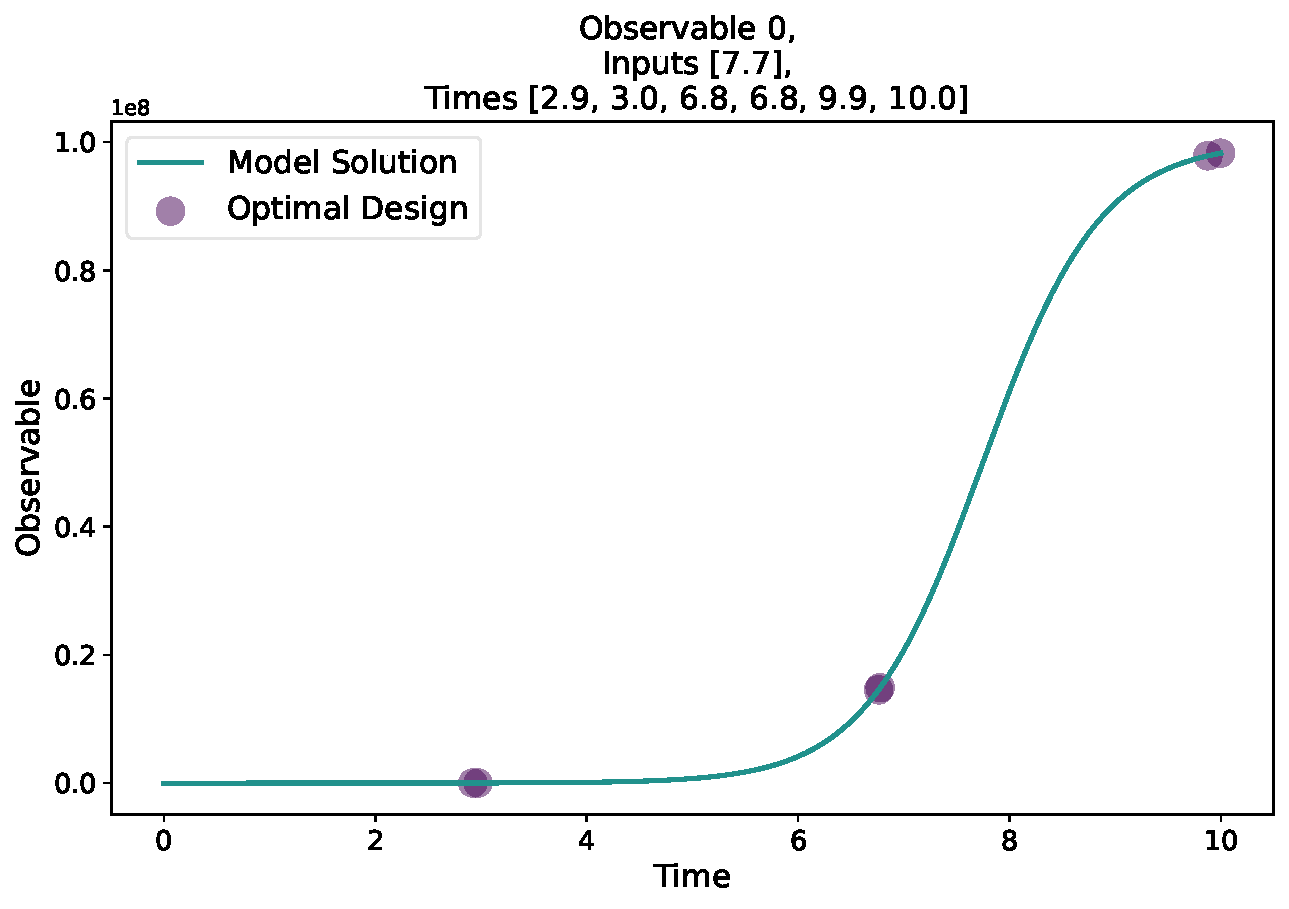
\includegraphics[scale=0.4]{Figures/Observable_Results_baranyi_roberts_ode_fisher_determinant_rel_sensit_cont_6times_1temps_000_x_00.pdf}
    \caption{{\footnotesize The example of the output of the Experimental Design optimization procedure for the Baranyi and Roberts model. 
    The line plot presents the model solution for the observable, and the scatter plot determines the time points chosen by Experimental Design.}}
    \label{fig:baranyi_roberts_observable}
\end{figure}
As can be noticed, the algorithm chooses three different time points.
Each of these time points corresponds to an extreme of one sensitivity meaning that we obtained one time point for each parameter.
The times 2.9 and 3.0 sample the lag-phase, where the growth still did not start.
The value 6.8 characterizes the growth rate of the model.
Finally, the measurement times 9.9 and 10.0 are responsible for the saturation phase $x_1^\text{max}$.
\begin{figure}[H]
    \begin{subfigure}{.9\textwidth}
      \centering
      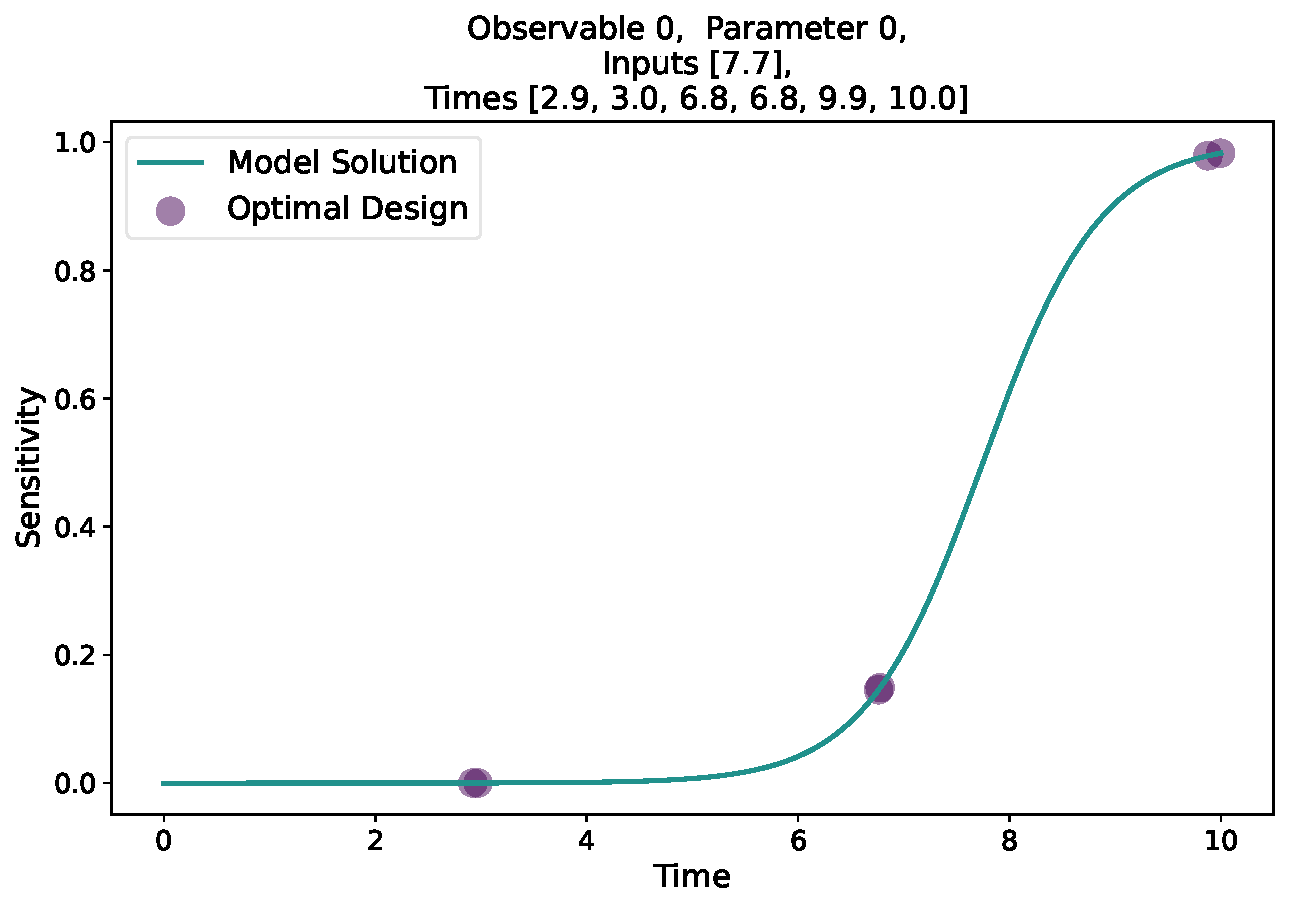
\includegraphics[scale=0.35]{Figures/Sensitivity_Results_baranyi_roberts_ode_fisher_determinant_rel_sensit_cont_6times_1temps_000_x_00_p_00.pdf}
    \end{subfigure}
    \begin{subfigure}{.9\textwidth}
      \centering
      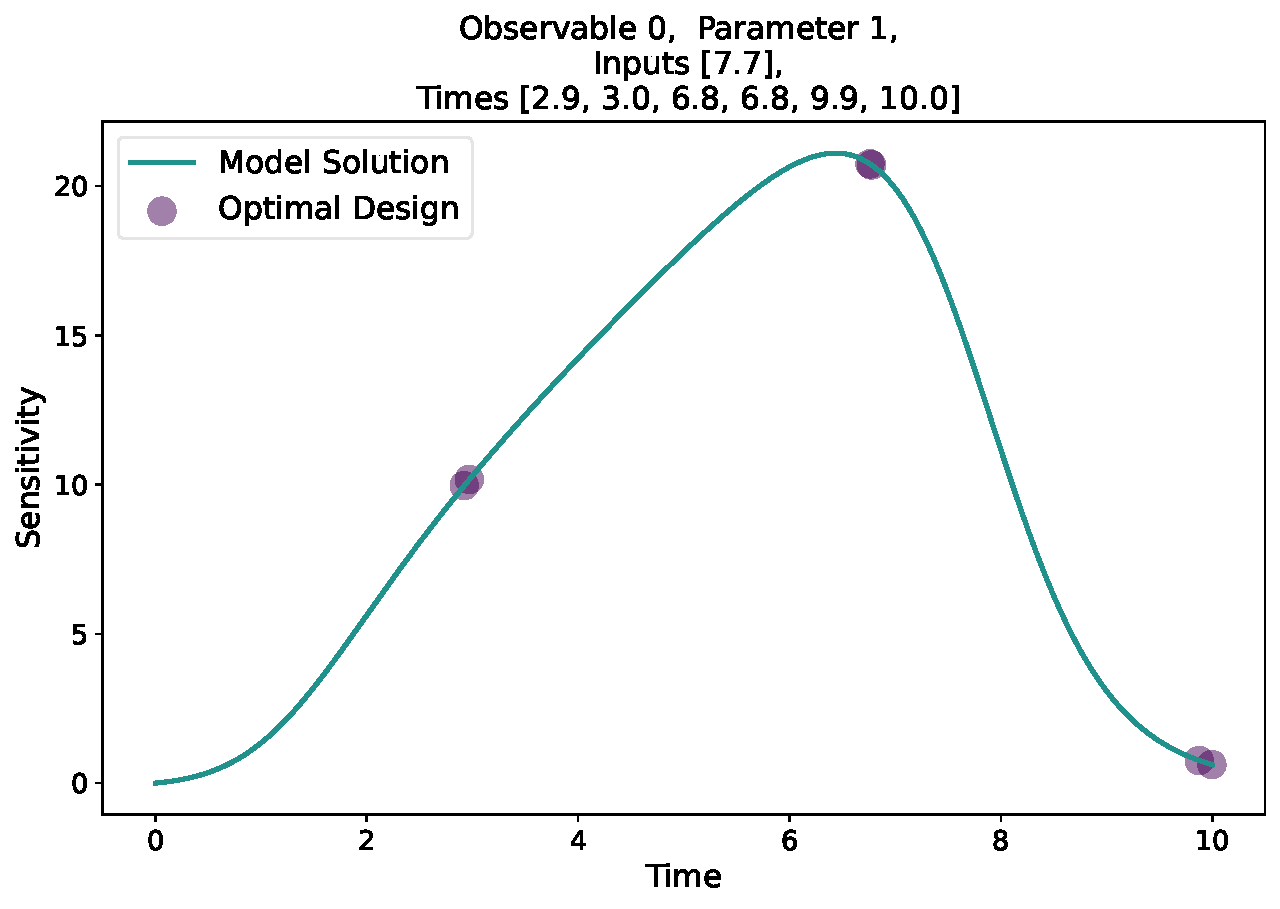
\includegraphics[scale=0.35]{Figures/Sensitivity_Results_baranyi_roberts_ode_fisher_determinant_rel_sensit_cont_6times_1temps_000_x_00_p_01.pdf}
    \end{subfigure}

    \begin{subfigure}{.9\textwidth}
        \centering
        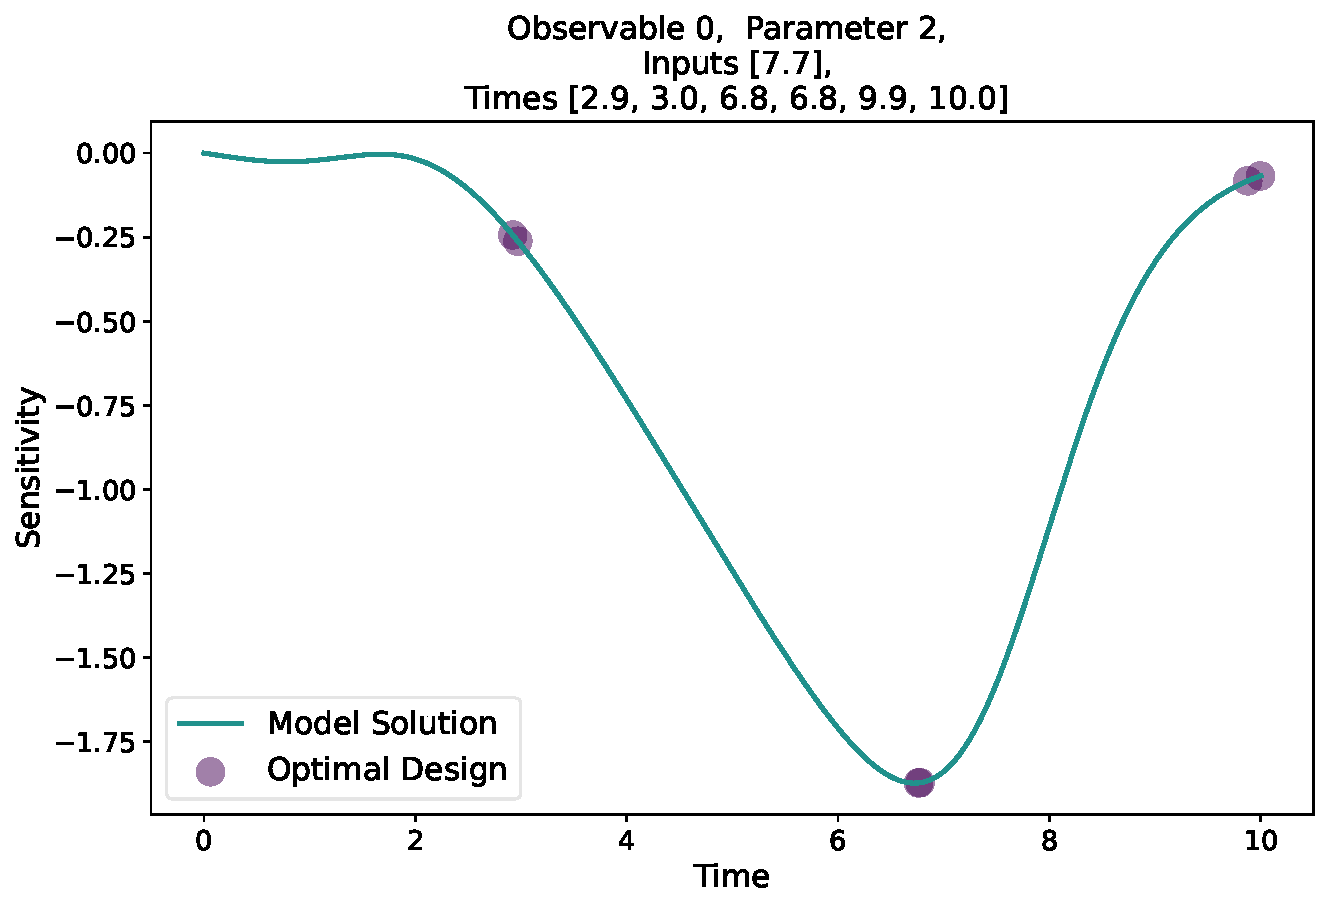
\includegraphics[scale=0.35]{Figures/Sensitivity_Results_baranyi_roberts_ode_fisher_determinant_rel_sensit_cont_6times_1temps_000_x_00_p_02.pdf}
    \end{subfigure}
    \caption{{\footnotesize The example of the sensitivities calculated for the Experimental Design optimization procedure for the Baranyi and Roberts model.
    The line plots present the model solution for the sensitivitied, and the scatter plots determine the time points chosen by Experimental Design.}} 
    \label{fig:baranyi_roberts_sensitivities}
    \end{figure}

Based on the results of the Experimental Design, one may claim that the optimal number of measurement times is 3.
Indeed, consider how the determinant increases with the number of measurement times in the logarithmic scale (see Fig. \ref{fig:det_vs_ntimes}).
It can be noticed that the slope of the curve between values 2 and 3 is much more significant (approximately fifteen orders of magnitude) than in the case of the further increase of measurement points.
For a higher number of times, informational profit stays at the same order of magnitude.
As a result, the researcher can significantly reduce the experimental workload without a noticeable loss of information.
\begin{figure}[H]
    \centering
    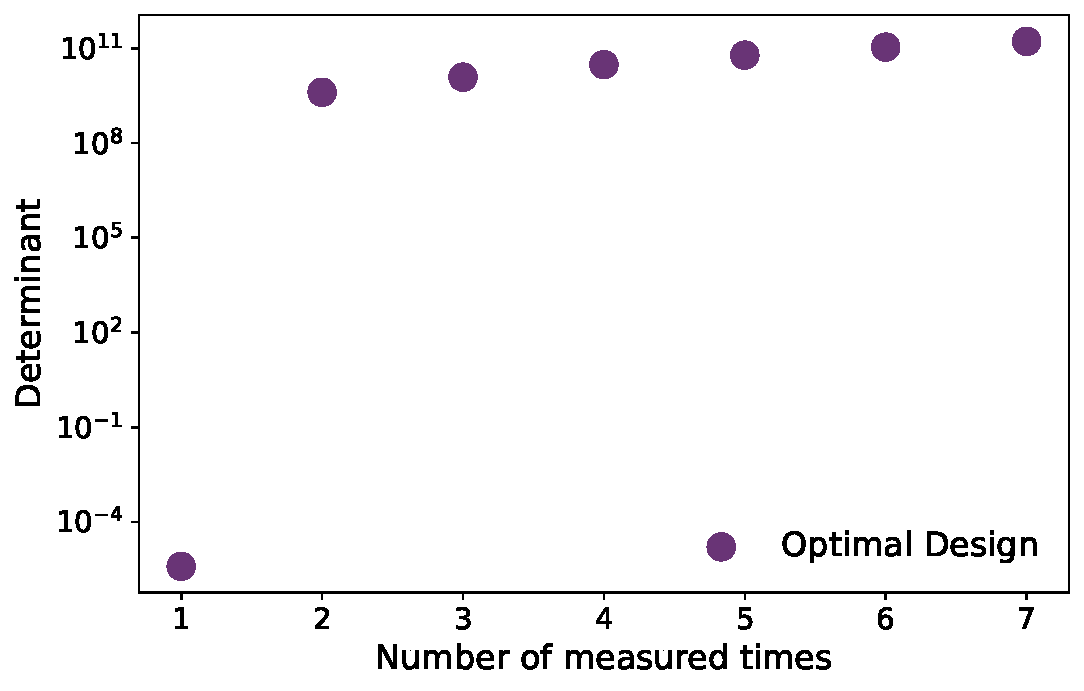
\includegraphics[scale=0.4]{Figures/det_vs_ntimes.pdf}
    \caption{{\footnotesize The determinant of the Fisher information matrix as a function of the number of measurement times.}}
    \label{fig:det_vs_ntimes}
\end{figure}
%
%
%
% ########################################################################
% ########################################################################
\section*{Supporting information}
%
%
%
\nolinenumbers
% ########################################################################
% ########################################################################
\bibliography{predictive-microbiology-software}

\end{document}
